\documentclass[a4paper,12pt]{article}
\usepackage[utf8]{inputenc}
\usepackage{geometry}
\usepackage{fancyhdr}
\usepackage{xcolor}
\usepackage{minted}
\usepackage{graphicx}
\usepackage{hyperref}
\usepackage{enumitem}
\usepackage{tikz}
\usetikzlibrary{shapes, arrows, arrows.meta, positioning, shadows, fit, calc, shapes.multipart}

% Geometry setup
\geometry{top=2.5cm, bottom=2.5cm, left=2.5cm, right=2.5cm}

% Header and Footer
\pagestyle{fancy}
\fancyhf{}
\lhead{\textbf{CMP9134: Software Engineering}}
\rhead{\textbf{Week 5}}
\lfoot{University of Lincoln}
\rfoot{Page \thepage}

% Color definitions
\definecolor{lightgray}{rgb}{0.95,0.95,0.95}

\begin{document}

%----------------------------------------------------------------------------------------
%   TITLE SECTION
%----------------------------------------------------------------------------------------

\begin{center}
    \LARGE \textbf{Lab Sheet 5: Architecture, Patterns \& Reuse} \\
    \vspace{0.5cm}
    \large \textbf{Objectives}
\end{center}

\noindent By completing today's workshop, you will:
\begin{itemize}
    \item Define the high-level \textbf{Architectural Pattern} for your Ground Control Station.
    \item Apply a \textbf{Design Pattern} (Singleton or Facade) to your Robot API client code.
    \item Perform an \textbf{Open-Source License Audit} on your dependencies to ensure legal compliance.
    \item Define the \textbf{Provides and Requires Interfaces} for a core system component using CBSE principles.
\end{itemize}

\vspace{0.5cm}
\hrule
\vspace{0.5cm}

\section*{Introduction: Bridging Design and Implementation}
You have gathered your requirements, mapped your models, and set up your Agile board. Now, you are transitioning into implementation. Before you start writing thousands of lines of code, you must decide \textit{how} that code will be organized (Architecture) and \textit{how} you will solve recurring coding problems (Design Patterns). Because you are building this system using modern frameworks, you will also heavily rely on Software Reuse (Open Source).



\vspace{0.4cm}
\textbf{Example:}
\begin{center}
\resizebox{\textwidth}{!}{
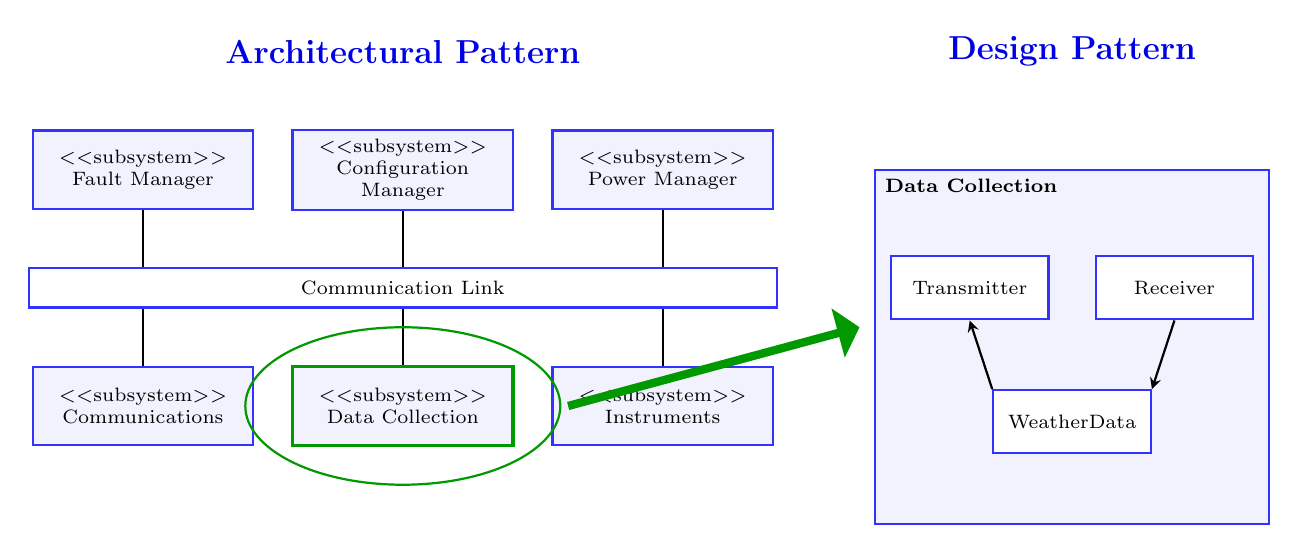
\begin{tikzpicture}[
    % Styles
    subsystem/.style={rectangle, draw=blue!80, fill=blue!5, thick, minimum width=2.8cm, minimum height=1cm, align=center, font=\scriptsize},
    bus/.style={rectangle, draw=blue!80, fill=white, thick, minimum width=9.5cm, minimum height=0.5cm, align=center, font=\scriptsize},
    designbox/.style={rectangle, draw=blue!80, fill=white, thick, minimum width=2cm, minimum height=0.8cm, align=center, font=\scriptsize},
    arrow/.style={->, >=stealth, thick}
]

    % --- Left Side: Architectural Pattern ---
    \node[font=\large\bfseries, text=blue!90!black] at (1.5, 2.5) {Architectural Pattern};
    
    % Top row subsystems
    \node[subsystem] (fm) at (-1.8, 1) {$<<$subsystem$>>$\\Fault Manager};
    \node[subsystem] (cm) at (1.5, 1) {$<<$subsystem$>>$\\Configuration\\Manager};
    \node[subsystem] (pm) at (4.8, 1) {$<<$subsystem$>>$\\Power Manager};
    
    % Communication Bus
    \node[bus] (link) at (1.5, -0.5) {Communication Link};
    
    % Bottom row subsystems
    \node[subsystem] (comm) at (-1.8, -2) {$<<$subsystem$>>$\\Communications};
    \node[subsystem, draw=green!60!black, very thick] (dc) at (1.5, -2) {$<<$subsystem$>>$\\Data Collection};
    \node[subsystem] (inst) at (4.8, -2) {$<<$subsystem$>>$\\Instruments};
    
    % Connections to bus
    \draw[thick] (fm.south) -- (fm.south |- link.north);
    \draw[thick] (cm.south) -- (cm.south |- link.north);
    \draw[thick] (pm.south) -- (pm.south |- link.north);
    \draw[thick] (comm.north) -- (comm.north |- link.south);
    \draw[thick] (dc.north) -- (dc.north |- link.south);
    \draw[thick] (inst.north) -- (inst.north |- link.south);
    
    % Circle around Data Collection to emphasize the zoom
    \draw[green!60!black, thick] (1.5,-2) ellipse (2cm and 1cm);

    % --- Right Side: Design Pattern ---
    \node[font=\large\bfseries, text=blue!90!black] at (10, 2.5) {Design Pattern};
    
    % The zoomed-in package box
    \draw[thick, draw=blue!80, fill=blue!5] (7.5, -3.5) rectangle (12.5, 1);
    \node[anchor=north west, font=\scriptsize\bfseries] at (7.5, 1) {Data Collection};
    
    % Internal classes (Design Pattern)
    \node[designbox] (trans) at (8.7, -0.5) {Transmitter};
    \node[designbox] (recv) at (11.3, -0.5) {Receiver};
    \node[designbox] (weather) at (10, -2.2) {WeatherData};
    
    % Internal connections
    \draw[arrow] (weather.north west) -- (trans.south);
    \draw[arrow] (recv.south) -- (weather.north east);

    % --- Connecting Arrow (Zoom effect) ---
    \draw[-{Triangle[width=18pt,length=8pt]}, line width=3pt, draw=green!60!black, fill=green!60!black] (3.6, -2) -- (7.3, -1);

\end{tikzpicture}
}
\end{center}
\vspace{0.4cm}

%----------------------------------------------------------------------------------------
%   OOP REFRESHER
%----------------------------------------------------------------------------------------

\section*{OOP Refresher for Beginners}
If you are new to programming, "Object-Oriented Programming" (OOP) might sound intimidating. However, it is just a way to organize your code so it is easier to read and reuse.
\begin{itemize}
    \item \textbf{Class (The Blueprint):} A class is like an architectural blueprint. It defines what something is and what it can do. (e.g., \texttt{class RobotClient}).
    \item \textbf{Object / Instance (The House):} When you actually build a house from the blueprint, that is an "Object" or an "Instance." You can only have one blueprint, but you can build many houses from it.
    \item \textbf{Attributes (The Data):} Variables stored inside the class\\ (e.g., \texttt{api\_url = "http://localhost:5000"}).
    \item \textbf{Methods (The Actions):} Functions written inside the class (e.g., \texttt{def moveRobot(x, y):}).
\end{itemize}
\textit{If you need a deeper dive into these concepts before starting Task 2, please check the "Beginner OOP Resources" section at the end of this document!}

%----------------------------------------------------------------------------------------
%   TASK 1
%----------------------------------------------------------------------------------------

\section*{Task 1: Mapping Your Architectural Pattern}

\textbf{Goal:} Document the high-level organization of your software system.

\textbf{The Concept:} An architectural pattern provides a stylized description of good design practice. Whether you are using a Python/Flask backend with HTML templates, or a Node.js API with a React frontend, your system will likely follow a \textbf{Layered Architecture} or the \textbf{Model-View-Controller (MVC)} pattern.

\vspace{0.3cm}
\textbf{Action:}
\begin{enumerate}
    \item In your GitHub repository, create or open your \texttt{ARCHITECTURE.md} file.
    \item Write a brief section (1-2 paragraphs) declaring your chosen tech stack and mapping it to an architectural pattern.    \textit{Look at the resource section below for examples of other Architectural Patterns in case you want to explore something different.}
    \item Answer the following questions based on your specific implementation:
    \begin{itemize}
        \item \textbf{If using MVC:} What framework handles the \textit{View} (renders the UI)? What handles the \textit{Controller} (processes HTTP requests and logic)? What acts as the \textit{Model} (database/business logic)?
        \item \textbf{If using Layered:} What libraries compose your Data Access layer? What comprises your User Interface layer?
        \item \textbf{If using a different pattern or using a combination of patterns (yes, you can!):} Describe the layers/components of your architecture and their responsibilities.
    \end{itemize}
    \item \textit{Tip: Use Mermaid.js from last week to sketch a quick diagram of these layers/components!}
\end{enumerate}
    
 

%----------------------------------------------------------------------------------------
%   TASK 2
%----------------------------------------------------------------------------------------

\section*{Task 2: Applying a Design Pattern in Code}

\textbf{Goal:} Use a low-level design pattern to solve a software construction problem.

\textbf{The Concept:} Your dashboard must communicate with the Virtual Robot via a REST API. You should not sprinkle raw HTTP requests (like \texttt{fetch} or \texttt{requests.post}) randomly throughout your codebase. Instead, you should create a dedicated "Robot API Client" class.
\begin{itemize}
    \item \textbf{The Facade Pattern:} This class acts as a Facade, hiding the messy HTTP headers, JSON parsing, and error handling behind clean methods like \texttt{moveRobot(x, y)}.
    \item \textbf{The Singleton Pattern:} You only want \textit{one} instance of this API client managing the connection across your entire app.
\end{itemize}

\vspace{0.3cm}
\textbf{Action:}
\begin{enumerate}
    \item In your codebase, create a new file for your Robot API Client (e.g., \texttt{RobotClient.py}, \texttt{robotService.js}, \texttt{RobotAPI.java}, depending on your language).
    \item Research how to implement the \textbf{Singleton Pattern} in your chosen language. 
    \item Write the "stub" (the class definition and empty methods) for this client. Ensure it implements the Singleton pattern so it cannot be instantiated more than once.
    \item Add placeholder methods for the Facade operations: \texttt{getStatus()}, \texttt{move(x, y)}, and \texttt{reset()}.
\end{enumerate}

%----------------------------------------------------------------------------------------
%   TASK 3
%----------------------------------------------------------------------------------------

\section*{Task 3: Open-Source License Audit (LEPSI)}

\textbf{Goal:} Practice safe software reuse by evaluating the legal constraints of your dependencies.

\textbf{The Concept:} The developer of open-source code still legally owns it and places restrictions on how it is used via licenses. Permissive licenses (MIT, Apache) allow you to do almost anything, while Copyleft licenses (GPL) force your project to adopt the same open-source rules. You must verify you are not violating these terms.



\vspace{0.3cm}
\textbf{Action:}
\begin{enumerate}
    \item Identify 3 to 5 third-party libraries/frameworks you plan to reuse in your project (e.g., React, Express, Flask, SQLite, Axios, Bootstrap).
    \item Visit their official GitHub repositories or websites to find their \texttt{LICENSE} file.
    \item Create a table in your documentation (or draft it for your final report) listing:
    \begin{itemize}
        \item Component Name
        \item Purpose in your system
        \item License Type (e.g., MIT, Apache 2.0, GPLv3)
        \item Is it Permissive or Copyleft?
    \end{itemize}
    \item Write a one-sentence conclusion stating whether your current combination of licenses imposes any legal restrictions on your Ground Control Station.
\end{enumerate}

%----------------------------------------------------------------------------------------
%   TASK 4
%----------------------------------------------------------------------------------------

\section*{Task 4: CBSE Interface Specification}

\textbf{Goal:} Define a system component as an independent service provider using Component-Based Software Engineering (CBSE) principles.

\textbf{The Concept:} In CBSE, components are abstract, stand-alone entities specified entirely by their interfaces. The \textbf{Provides interface} defines the services the component offers, while the \textbf{Requires interface} defines the external services it needs to execute.

\vspace{0.3cm}
\textbf{Action:}
\begin{enumerate}
    \item Your assessment requires a \textbf{Mission Logger} to create an audit trail of user commands. Let's treat this as an independent CBSE component.
    \item Open a markdown file or a diagramming tool.
    \item Define the \textbf{Provides Interface} for the Mission Logger. What methods/services will it expose to the rest of your backend? (e.g., \texttt{logCommand(user, action)}, \texttt{exportLogs()}).
    \item Define the \textbf{Requires Interface}. What external services does the Logger need to function properly? (e.g., \texttt{Database Connection}, \texttt{System Clock/Timestamp Service}).
    \item \textit{Stretch:} Sketch this out using the UML "ball and socket" notation demonstrated in the lecture.
\end{enumerate}

%----------------------------------------------------------------------------------------
%   RESOURCES
%----------------------------------------------------------------------------------------
\section*{Further Resources}

\textbf{Beginner OOP Resources:}
\begin{itemize}
    \item \textbf{Python OOP for Beginners (Real Python):} \href{https://realpython.com/python3-object-oriented-programming/}{realpython.com/python3-object-oriented-programming/} - \textit{An easy-to-read guide on how to create classes and objects in Python.}
    \item \textbf{JavaScript Classes (MDN Web Docs):} \href{https://developer.mozilla.org/en-US/docs/Learn/JavaScript/Objects/Classes_in_JavaScript}{developer.mozilla.org/.../Classes\_in\_JavaScript} - \textit{The official beginner's guide to writing OOP in modern JavaScript/Node.js.}
\end{itemize}

\textbf{Architecture \& Design Patterns:}
\begin{itemize}
    \item \textbf{\href{https://github.com/mehdihadeli/awesome-software-architecture}{https://github.com/mehdihadeli/awesome-software-architecture}} - \textit{A curated list of software architecture resources and patterns.}
    \item \textbf{Refactoring.Guru (Design Patterns):} \href{https://refactoring.guru/design-patterns}{https://refactoring.guru/design-patterns} - \textit{Excellent resource with code examples for Singletons and Facades in almost every language.}
    \item \textbf{ChooseALicense.com:} \href{https://choosealicense.com/}{https://choosealicense.com/} - \textit{A simple guide to understanding the legal implications of Open Source licenses.}
    \item \textbf{MVC Pattern Explained:} \href{https://developer.mozilla.org/en-US/docs/Glossary/MVC}{MDN Web Docs: MVC}
\end{itemize}

\end{document}

\end{document}